\documentclass{llncs}
%
\usepackage{graphicx}
\DeclareGraphicsExtensions{.eps}

\newcommand\ignore[1]{}
\newcommand{\imagepathext}[5]{%
\begin{figure}[!htbp]
\hfil\includegraphics[#1]{#2/#3.#4}\hfil
\caption{#5\label{#3}}
\end{figure}}

\newcommand{\image}[3]{\imagepathext{#1}{pics}{#2}{eps}{#3}}
\newcommand{\png}[2]{\imagepathext{width=\columnwidth}{pics}{#1}{png}{#2}}


%

\begin{document}

\frontmatter          % for the preliminaries
\pagestyle{headings}  % switches on printing of running heads
\mainmatter              % start of the contributions
%
\title{A Low-cost Natural Interaction based on a Camera Hand-Gestures Recognizer}
\author{Mohamed-Ikbel Boulabiar\inst{1} \and Thomas Burger\inst{2}
Franck Poirier\inst{3} \and Gilles Coppin\inst{1}}
%
\institute{LAB-STICC, Telecom-Bretagne, France,\\
\email{boulabiar@gmail.com, gilles.coppin@telecom-bretagne.eu},
\and
LAB-STICC, University of Bretagne-Sud, France
\email{thomas.burger@univ-ubs.fr}
\and
VALORIA, University of Bretagne-Sud, France
\email{franck.poirier@univ-ubs.fr}
}

\maketitle

\begin{abstract}
The search for new simplified interaction techniques is always treated as a
manner to advance the communication with interactive devices.
In this paper, we present our work to generate interactive TVs modules capable
of recognizing human gestures through the PS3Eye low-cost camera.
We recognize gestures by the tracking of human skin blobs and analyzing the 
corresponding movements to control a TV in an ubiquitous computing environment.
We also present a new free gestures icons library created to allow easy
representation and diagramming.
%after an analysis of TV's Talk-shows.

\keywords{natural gesture interaction, low-cost gesture recognition, interactive
TV broadcast, ubiquitous computing}
\end{abstract}
%

\section{Introduction}
HCI research focuses more attention than before on enhancing the user experience
regarding human-display interaction in order to interact more naturally without
the need of clicking on buttons and touching screens. However, in everyday life
interaction with home devices having embedded computational power, such as
interactive TVs, one does not make benefit of these new interaction paradigms yet. 

We present in this paper an approach that could allow the detection and the
interpretation of gestures of a TV spectator from a simple and low cost camera. 
RevTV is the name of the French project for adding new interaction techniques
to TVs to allow the inclusion of the telespectator.
%The final objective of this study is to control the animations of an avatar
%that should be inserted within a TV show beside the presenter or actor [RevTV].
Its major scenario which we rely on, corresponds to educational games where a
pupil controls his/her avatar in a program led by a ``real'' TV animator.
This kind of scenarios needs to be able to manage commands interaction
like pointing, selecting and moving as well as natural gesture animation.


\section{Gesture Semantics}
Gestures do not come alone, they are combined with speech, or with cognitive
activity. We study in this part the sources of gestures and the relation between
them and other activities.
First sources of gestures can come from the interaction between two human in a
discussion, these type of gestures are used to add more precision on the details
and they are made by the same auditory areas of the cortex \cite{SymbolicGest}.

Semantics of gestures have been also studied by the analysis of the movements of
a user explaining a story \cite{gestureThought}.
These gestures are called gesticulations and are always accompanying a speech. 

This semantics can be divided into two parts:
\begin{description}
 \item[Animation Gestures] used to animate a virtual avatar.
 \item[Command Gestures] used to launch a specific predefined action.
\end{description}


\ignore{
Gesture recognition got the attention of HCI researchers in order to find better
ways to talk to the computer. The first one was the Hand Gestural Cursor
(Put-That-There[]) aiming to the simplification of the means of communication
between human and the machine.
Since then, the gesture definition included more techniques and got applied on
the 2D recognition which is the multi-touch gestures.
}

\subsection{Gestures taxonomies}
By looking at the possible gestures human can generate \cite{Gesturecraft}, we
get a huge amount of possibilities which depend on the context and on the type.
%So, there is a need for a taxonomy.
%Many possible taxonomies exist according to the technical or analytical aspects:
%In order to describe and analyse each gesture, we can rely on the following aspects:
\ignore{\begin{description}
 \item[Gesture Creation Space:] We use this criteria to distinguish between gestures made in the 2D or 3D space.
 \item[Number of used strokes:] We use this criteria to distinguish between gestures constructed by only one path and between those using many paths, so the recognition needs to wait for all strokes before the recognition
 \item[Gesture context:] We use this criteria to distinguish gesture based on the specific use of it, gestures for disabled people, gestures in talk-shows, gestures in meetings.
\end{description}}
%Gesture and Thoughts, page 18
According to McNail \cite{gestureThought}, it is possible and useful to
distinguish between these gestures and a possbile taxonomy can provide us these
types:
\begin{description}
 \item[Gesticulation] is a motion that embodies a meaning reliable to the
accompanying speech. It is made chiefly with the arms and hands but is not
restricted to these body parts.
 \item[Speech-linked gestures] are parts of sentences themselves, the gesture
completes the sentence structure.
 \item[Emblems] are conventionalized signs, such as thumbs-up or the ring (first
finger and thumb tips touching, other fingers extended) for ``OK.''
 \item[Pantomime] is dumb show, a gesture or sequence of gestures conveying a
narrative line, with a story to tell, produced without speech.
\end{description}

In our work, we focalize on emblems commands and gesticulations.
%We have chosen to analyze gesticulations as they are the most frequent.
%, and project them on the technical taxonomies.
%And we have also made our own extraction from Talk-Shows.
%Nous avons choisi celle-ci, car elle correspond aux besoins que nous avons identifier dans les scenarios d'utilisation de la télé interactive

\subsection{Gestures Library}

In order to identify relevant gestures we have analyzed some talk-shows in order
to extract most frequent gestures being performed.
According to our scenario of use in the context of Interacrive TV.
%and defining a benchmark scenario.
%We have tried to target the following kinds of gestures in a first step.

\png{handg}{Family of supported gestures}

Fig.\ref{handg} shows our supported gestures. We provide a movement mode
used to select the 4 directions, then a multitouch nthen a command mode, then a hand fingers recognition,
and, finally, a cursor movement mode.
%\pagebreak 
We have selected 4 basic gestures modes to be supported in our system as a first step.
Then to be extended depending on the context fulfilling the requirements
of our scenario.

\section{Technical Work}

In the figure \ref{pipeline}, we show the pipeline of the modules used to
extract gestural informations. Each part is described in details in the next
subsections.

\png{pipeline}{Pipeline of work components}


\subsection{Used Materials}
We have chosen a low-cost camera for our work that can be integrated with other components in the future.
The PS3Eye camera matched our expectations with a 640x480 resolution combined with a 60 frames-per-second capability.
This camera costs about 40\$, which is a reasonable price for a potential market deployment.

\subsection{Color Transformations}
The video processing is based on several modules.
First, a basic but adaptive skin color segmentation of a large interval of human skin varieties is performed \cite{skinColorSeg}.
We also use a histogram equalisation technique to better enlarge the colors to all the space available.
Then we transform the color space from BGR, which come from the camera to YCrCb,
as it’s the most adapted one to skin segmentation
Moreover, the corresponding transformation is linear \cite{skinColorSeg}.

Other color spaces like HSV or CIE-Lab can be used for skin color segmentation,
but the transformation from BGR either takes more time or needs more parameters
in the next step.

\begin{center}
\begin{tabular}{|l|c|c|c|c|}
\hline
\textbf{Space} & BGR & HSV & YCrCb & CIE Lab\\
\hline
 & R\textgreater 95, G\textgreater 40, B\textgreater 20, & H[0.4 .. 0.7] & Cb[77 .. 127] & C[0 .. 65] \\
\textbf{Param.} & Max\{R,G,B\}-Min\{R,G,B\}\textless 15 & S[0.15 .. 0.75] & Cr[133 .. 173] & I[0 .. 14] \\
 & abs(R-G)\textgreater 15, R\textgreater G, R\textgreater B & V[0.35 .. 0.95] & & \\
\hline
\end{tabular}
\end{center}

\subsection{Input Filtering}
During this step, a 5x5 opening morphological kernel \cite{morphologicalAnalysis} is applied to smooth the results,
this is necessary to clean the image from isolated pixels and holes inside skin
zones.

\subsection{Blobs Detection}
Each blob is labeled in linear time using the contour tracing technique with
the linear-time component-labeling algorithm \cite{CompLabeling},
which requires 1 to 4 passes to recognize all blobs with their bounding contour.
We identify the hands and the head by a calibration focused on their first
position in the screen. We identify them and add a tag to their respective blobs.

%Fig. Skin segmentation
% Testing graphics
\png{skincolor}{Skin color}
\section{Blobs Tracking}
After having the hands and head blobs identified, an efficient
tracking method based on the apparence model for occlusion handling\cite{app06}.
We have used the cvblob implementation \cite{cvblob} for that algorithm which 
stores the mesures of bounding boxes distance and provide tracks instead of just blobs.  %distantBlobTrack.

When the matrix of distance is set up, the coming loops
are executed to handle blobs changes:
\begin{itemize}
 \item A loop to detect inactive tracks: those tracks with no blobs near.
 \item Detect and create new tracks: those blobs without a track near.
 \item A loop to assign blobs to tracks. It makes clusters with blobs that are close and assign them to a track.
In this step some tracks could merge in one.
 \item A last loop which check all inactive tracks to delete the old ones.
\end{itemize}

To better handle blobs, the bounding path of the blobs
is simplified to a set of few points when needed.
This is used to identify picks for the counter mode.

\section{Gestural informations and Recognition modes}
The output of the video processing is the input of the recognition module,
which is based on the track location on the screen.
Four different modes are defined according to the hand locations. The switch between them is based on the following grammar:
\begin{description}
 \item[The movement mode:] it is activated when two hands are close to each other, so that the user selects between 4 directions. This mode can be used as input for games to select between the directions.
 \item[The multi-touch mode:] where we consider the similarities between 2D gestures in a tactile multi-touch context and gestures in the 3D space. To do so, we consider the hands blobs in a manner similar to that of two finger tips in the input of a multi-touch device. Based on that, we can recognize well known multi-touch gestures, such as Drag, Pinch/Zoom and Rotate but applied on our case.
 \item[The counter mode:] counts the number of fingers in a preselected hand (the left and right hand are automatically discriminated) by counting the peaks in the simplified contour of the blob. This mode can again be used in games for kids.
 \item[The mouse mode:] it is used to control a cursor to select something in an arbitrary place on the screen. With this mode, we only get the input from a sub zone in the screen and map it to the full screen. We use it in a similar way to a computer touchpad.
The user can validate clicks using a tempo on another zone.
\end{description}

A phase of calibration is triggered when the logic of tracking is lost or damaged.
We have used four modes in a first core with the possibility to add more sub-gestures in the future.
This core will be used to control a children game having to select, choose, and answer basic questions.
We have stick to that scenario to produce these gestures. 

%\pngl{point}{simplify}{List of modes}

\begin{figure}[!htb]
\centering
  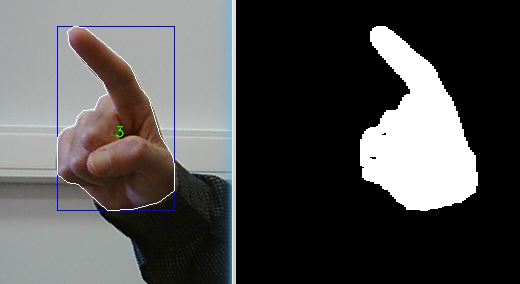
\includegraphics[width=0.45\textwidth]{./pics/point.png}
  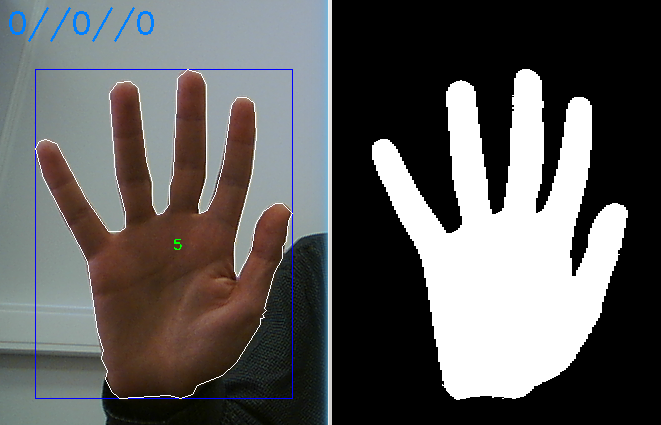
\includegraphics[width=0.4\textwidth]{./pics/simplify.png}
  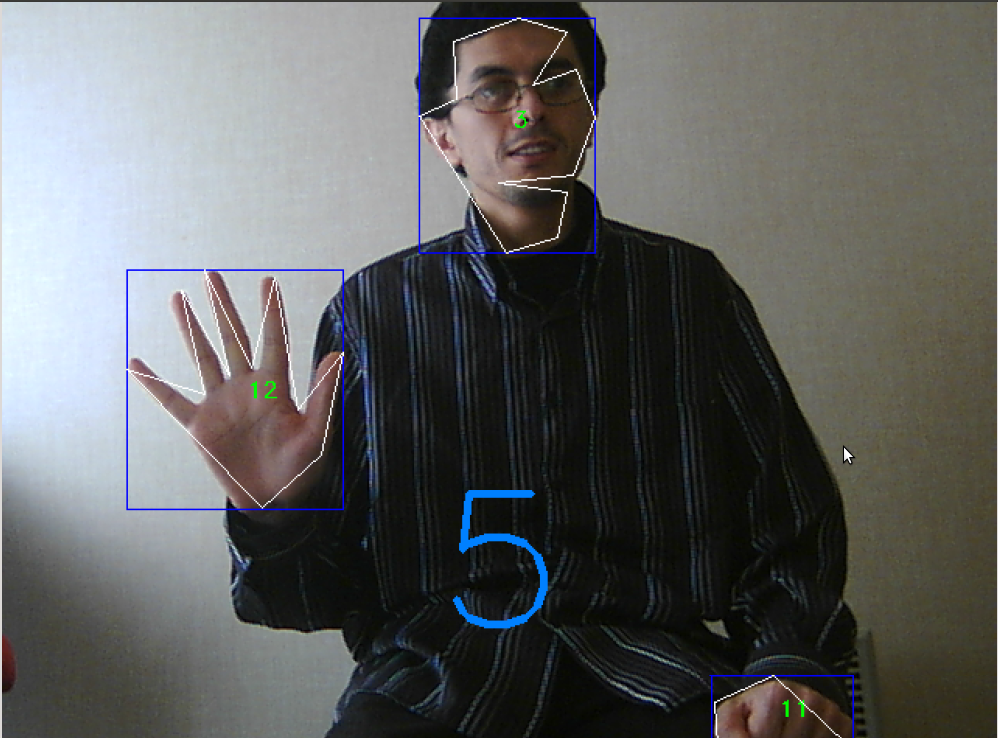
\includegraphics[width=0.46\textwidth]{./pics/fingers.png}
  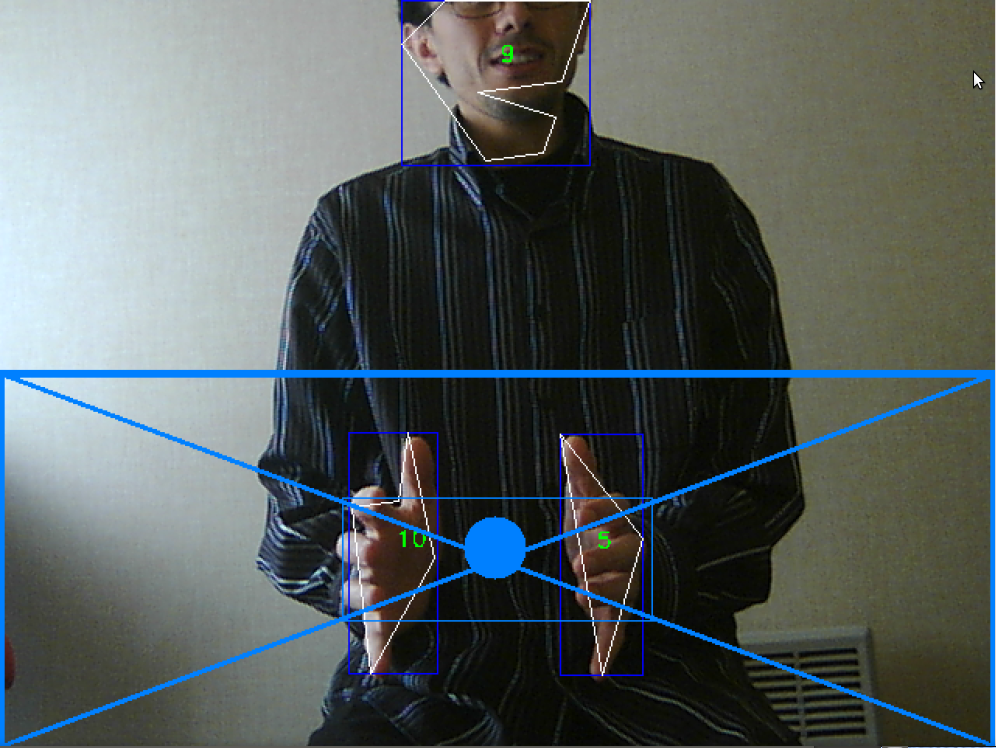
\includegraphics[width=0.46\textwidth]{./pics/move.png}
  \caption{List of modes}
%  \label{fig:Gestes}
\end{figure}


\section{Usability and Naturalness in an ubiquitous environment}

The usability of our system should be compared to other systems in an ubiquitous
environment. In our case, we have a TV instead of a PC.
The gestures in such environment, and specially for children game scenario,
are made for a short period of time, and doesn't require a good usability,
even if we can recognize gestures in real-time.

The Naturalness of gestures is supported by the analysis of those to be
supported and the choice of gesticulation.
Gesticulation are the most common ones, so they inherit from this their
ability to be produced with less complication.

Emblems gestures which englobe commands, are choisen to be produced in more
difficult positions to allow easy descrimination from gesticulations.

Spacial gestural interactions always lack from the feedback for the interaction.
This affects also the usability because the user can no more be guided in space
as he was with surface movement or simple physical joysticks.

\section{System integration of this interaction and future work}

Our system support gestural interaction at the moment but other multimodal ways
to fine tune the input and give the user feedback are possible.
These possible evolution of the system are possible:

\begin{description}
 \item[Facial Recognition]: our system don't take care of the facial expressions
recogntions. A future support in this area can be added for more reactiveness in
pupil's games.
 \item[Voice Recognition]: To speed up commands handling, we can use short voice
keywords either to move from one mode to another, or to select object.
 \item[Haptic feedback]: A special wearable vest can be used to allow more
reactiveness with the user. But this area still lacking innovation because the
haptic feedback is by area and not continue.
\end{description}

\ignore{
Gesture + facial recog.
Voice recognition
Haptic 
--
Naturalness came from the analysis of gestures used in talk shows.
(gestures used many times means nature gestures)
Reverse thinking.
Usability in the context of RevTV ??
}
% ---- Bibliography ----
\bibliographystyle{splncs03}
\bibliography{paper}

\end{document}
